   \markboth{}{}
\begin{center}
	\Large \textbf{Referências}
\end{center}
	
[1] ELETROBRÁS. Diretrizes para estudos e projetos de Pequenas Centrais Hidrelétricas. Eletrobras, 2000.

[2] WISSMANN, Leandro; GRANDO, Maurício Nelson. Estudo prévio da instalação de uma pequena central hidrelétrica no manancial do rio Pato Branco no estado do Paraná. 2012. Trabalho de Conclusão de Curso. Universidade Tecnológica Federal do Paraná - Disponível em: \url{http://repositorio.roca.utfpr.edu.br/jspui/handle/1/442}

[3] ABREU, Thiago Modesto de. Proposta de Metodologia para definição de quantidade de grupos geradores de pequenas centrais hidrelétricas. 2015. Disponivel em: \url{http://www.aneel.gov.br/documents/656835/14876412/Disserta%C3%A7%C3%A3o+Thiago+Abreu+2015.pdf/7d05c97f-4e45-054c-33c6-020884240fef}

[4] Mapa de linhas de transmissão e subestações - Sistema Interligado Nacional - Rede de Operação. Disponível em:  \url{http://sindat.ons.org.br/SINDAT/Home/ControleSistema}

[5] Características e requisitos técnicos básicos das instalações de transmissão - Subestação Teixeira de Freitas 2. Disponível em: \url{http://www2.aneel.gov.br/aplicacoes/editais_transmissao/documentos/Lote_L_Anexo_T%C3%A9cnico_Eun%C3%A1polis_Teixeira_de_Freitas_II_C2.pdf}
	
[6] ANEEL, ANDEE. Atlas de energia elétrica do Brasil. Brasília, 2008.

[7] BRONZATTI, Fabricio Luiz; IAROZINSKI NETO, Alfredo. Matrizes energéticas no Brasil: cenário 2010-2030. Encontro Nacional de Engenharia de Produção, v. 28, p. 13-16, 2008.

[8] Revitalização da câmara de carga e do conduto forçado da usina hidrelétrica de rio branco do sul.Disponível em: \url{<http://repositorio.roca.utfpr.edu.br/jspui/bitstream/1/6766/1/CT_COELE_2015_1_14.pdf>}

[9] Energy Education. Disponível em: \url{<https://energyeducation.ca/encyclopedia/Spillway>}

[10] CUSSIOLI, Mariana Coppede. Dinâmica da desembocadura do rio Itanhém, Alcobaça, BA. 2010. Tese de Doutorado. Universidade de São Paulo - Disponível em: \url{<http://www.teses.usp.br/teses/disponiveis/21/21133/tde-14092012-133655/en.php>}

\newpage
\thispagestyle{empty}
\hfill
\vfill
\begin{center}
	\textbf{{\LARGE ANEXO}}
\end{center}

\vfill
\hfill

\newpage
\thispagestyle{empty}
\begin{landscape}
	\begin{figure}[h]
		\centering
		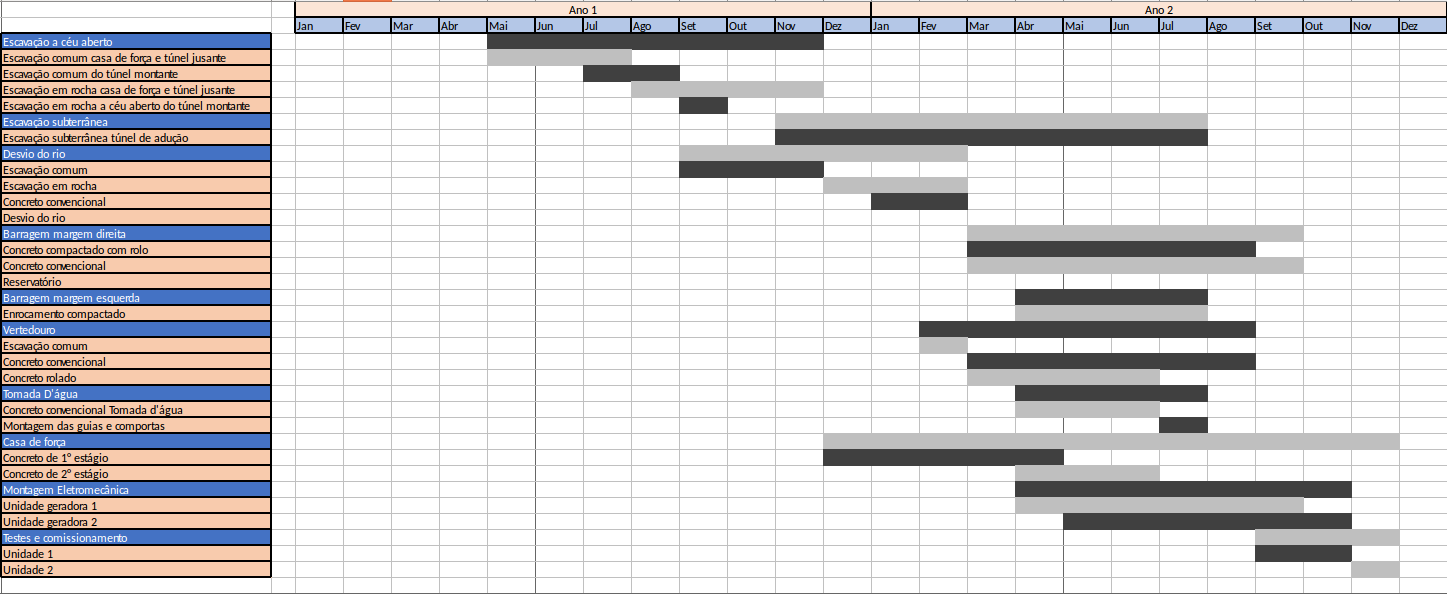
\includegraphics[width=1.6\textwidth]{cronos.png}
		\caption{Cronograma}
		\label{fig:cronos}
		\source{Cronograma do Projeto}
	\end{figure}
\end{landscape}
